\section{Basic Concepts of Optimal Experimental Design}
The initial setup of any experiment involves careful specifications of fundamental design concepts. The parameters of the process under study are considered as explanatory variables; each of them takes one value out of the set of possible values within the design region, i.e. the experiment is factorial. A combination of factors' levels defines a ``treatment'', or a ``design point'',  which might be used in a run of the experiment, and the set of all possible treatments will be referred to as the ``candidate set of treatments''. Theoretically this set can be infinite, however, in practice each factor has a finite number of levels, usually from $2$ to $5$, hence, the capacity of the candidate set is less than a few thousand points. For example, if a chemical reaction process is being investigated, possible variables may include temperature, pressure, presence or absence of catalysts, etc. Each of these parameters would be put to one out of a set of values, e.g. temperature may be equal to $20\degree$, $30\degree$, $50\degree$ or $60\degree$. Quite often (and throughout this thesis as well) the quantitative factors are scaled to $[-1,1]$ in order to ease the implementation of the design search and the interpretation of the results; the designs then are also presented using the scaled variables' values.

Each treatment that is used in the experiment is applied to at least one experimental unit -- an object or a collection of objects, indivisible in terms of treatment application and thus being considered as an elementary (primary) unit. One and only one treatment can be applied to each experimental unit and the structure of the population from which the sample of units has been taken should be explicitly comprehended. For example, in clinical trials when several drugs are compared, an individual person is often an experimental unit (so that each patient receives one drug). In industrial experiments a batch of material might be defined as a unit with treatments being different chemical applications; in agricultural experiments a single plant may be an experimental unit where, for example, plants are cultivated differently and then their productivity or growth performance is measured to compare the treatments \citep{MeadGilmour2012}. Units may be organised in a more complicated structure in order that a large portion of variability between them is eliminated: they can be gathered in blocks (then we have blocked designs), or nested within each other (multistratum experiments).

The allocation of treatments to units is arranged according to the concept of randomisation \citep{MeadGilmour2012}, that in a certain way allows minimising the impact of various uncontrolled (and often unknown) factors on the outcome of the experiment and provides the best chance of the statistically fair inferences being valid for the whole population of the experimental units.  

The main assumption underlying the experimentation is that there is a relationship of some form between the factors $(X_1,\ldots, X_k)$ $\in$ $\Theta \subset R^{k}$ and the response variable $Y=\eta(X_1,\ldots, X_k).$ 

Recall the polynomial regression model (\ref{eq::intro_model}) for the unblocked experiment, containing initial factors, their powers and interactions is used as a good approximation to the relation between the variables:  

\begin{equation}
\label{eq::back_model}
\bm{Y}=\bm{X\beta}+\bm{\varepsilon}.
\end{equation} 

Here $\bm{X}$ is the $n\times p$ model matrix, each row corresponds to a run of the experiment (experimental point), and each column to a term of the model (intercept, power of a factor or an interaction of powers of factors); $\bm{Y}$ is the $n\times 1$ vector of responses; $\bm{\beta}$ is the $p\times 1$ vector of parameters corresponding to the model terms and $\bm{\varepsilon}$ is the $n\times 1$ vector of independent normally distributed random error terms with constant variance, i.e. $\bm{\varepsilon}\sim \mathcal{N}(\bm{0},\sigma^{2}\bm{I}_{n})$. We do not take into consideration here possible systematic errors (e.g. an incorrectly configured measuring instrument or a device being incorrectly used by the experimenter) as they are outside the scope of statistics and cannot be discovered using statistical methods.   

The error variance estimation can be obtained in two ways. The first one is the mean square error: $\hat{\sigma}^2_{mse}=\mbox{Residual SS}/(n-p)$, i.e. the residual sum of squares divided by the corresponding number of degrees of freedom (obtained from the ANOVA decomposition, the details can be found in \cite{Draper1998}). This estimator obviously depends on the model and on the number of its parameters. The other one is model-independent `pure' error, derived from the further decomposition of the residual sum of squares into the `pure' error and `lack-of-fit' components: $\hat{\sigma}^2_{PE}=\mbox{Pure error SS}/(n-t)$, where $t$ is the number of unique treatments applied and $d=n-t$ is the pure error degrees of freedom, i.e. the number of replicated points. In other words, the error is estimated by fitting the full treatment model:

\begin{equation}
\label{eq::back_trnt}
\bm{Y}=\bm{X_{t}\mu_{t}}+\bm{\varepsilon},
\end{equation} 

where $\bm{X_{t}}$ is the $n\times t$ full treatment model matrix, in which the $(i,j)^{th}$ element is equal to $1$ if treatment $j$ is applied to the $i^{th}$ unit, otherwise it is set to $0$. Then the elements of the $t$-dimensional vector $\bm{\mu_{t}}$ are the mean effects of each treatment. The vector of errors $\bm{\varepsilon}$ comprises the between-unit variation, such that $\mbox{E}(\bm{\varepsilon})=\bm{0}$, $\mbox{Var}(\bm{\varepsilon})=\sigma^2\bm{I}_{n}$.

Many authors advocate the use of the `pure' error estimate of $\sigma^2$ instead of the one pooled with the lack-of-fit part from the model (\ref{eq::back_model}): \cite{Cox1958planning} recommends using it for the estimation unless there are no replicate treatments, while \cite{Draper1998} argue for the reliability of `pure' error and recommend aiming for the presence of replicates at the stage of planning. \cite{Atkinson2007} also state that ``If lack-of-fit of the model is of potential interest, $\sigma^{2}$ is better estimated from replicate observations'' (page 22). For response surface experiments in blocks \cite{Gilmour2000PErsm} explicated the definition of pure error and its estimate which are compatible with the unblocked case: from replicates but also taking into account  block effects additive to treatment effects. Finally, the work by \cite{GilmourTrinca2012} that inspired this research, comprises a thorough analysis in favour of estimating the error from the full treatment model which is true regardless of what function is used to approximate the relationship of interest.

\subsection{Primary criteria}
\label{seq::primary_criteria}
The objective underlying the model-fitting is obtaining quality estimates of the parameter vector $\bm{\beta}$. Their least squares estimators $\hat{\bm\beta}=(\bm{X}'\bm{X})^{-1}\bm{X}'\bm{Y}$ are unbiased and the variance-covariance matrix of the parameter estimations is $\mbox{Var}(\hat{\bm\beta})=\sigma^2(\bm{X}'\bm{X})^{-1}$, i.e. the error variance multiplied by the inverse of the Fisher information matrix. 
The volume of the joint $100(1-\alpha)\%$ confidence region for $\bm{\beta}$ is inversely proportional to $\vert\bm{X}'\bm{X}\vert^{1/2} / (F_{p,\nu;1-\alpha})^{p/2}$, where $F_{p,\nu;1-\alpha}$ is the $(1-\alpha)-$quantile of F-distribution with $p$ and $\nu$ degrees of freedom and $\nu$ is the number of degrees of freedom used for $\sigma^{2}$ estimation \citep{Draper1998}. If we use the residual mean square estimate of $\sigma^{2}$, the F-quantile does not depend on the design and we have standard $D$-criterion which is minimising $\vert(\bm{X}'\bm{X})^{-1}\vert$ \citep{Atkinson2007}. 

\citet{GilmourTrinca2012} considered the pure error estimation instead and derived the $DP$-criterion: minimising $(F_{p,d;1-\alpha_{DP}})^{p}\vert(\bm{X'}\bm{X})^{-1}\vert$. If only some of the parameters are of interest, it is possible to minimise the volume of a confidence region for a subset of parameters; corresponding $D_S$ and $DP_S$ criteria then will look as follows:
\begin{align*}
D_S: \mbox{minimise } &\vert [(\bm{X}'\bm{X})^{-1}]_{22}\vert, \\
DP_S: \mbox{minimise } &(F_{p_2,d;1-\alpha_{DP}})^{p_2}\vert [(\bm{X}'\bm{X})^{-1}]_{22}\vert,
\end{align*}
where $p_2$ is the number of parameters of interest and $[(\bm{X}'\bm{X})^{-1}]_{22}$ is the submatrix of the inverse of the information matrix that corresponds to the subset of interest.

Another widely used criterion considered here, the $L$-criterion, represents the mean of linear functions of the parameter estimates' variances. If we are interested in the functions of parameters given by $\bm{L}'\bm{\beta}$, then the variance-covariance matrix of $\bm{L}'\bm{\hat{\beta}}$ is $\bm{L}'(\bm{X}'\bm{X})^{-1}\bm{L}$. Due to the invariability of the trace under cyclic permutations, minimisation of the trace of $\bm{W}(\bm{X}'\bm{X})^{-1}$, where $\bm{W}=\bm{LL}'$, is equivalent to minimising the mean of the variances of these functions. If $\bm{W}$ is a multiple of the identity matrix, $L$-optimality is reduced to $A$-optimality (and to weighted $A$-optimality if all off-diagonal elements are zero). The $LP$-optimality criterion was defined by \citet{GilmourTrinca2012} as minimising  $F_{1,d;1-\alpha_{LP}}\mbox{tr}\{\bm{W}(\bm{X}'\bm{X})^{-1}\}$, that is minimising the mean of the squared lengths of confidence intervals for the linear functions defined by the columns of $\bm{L}$. In a similar way as before, $L_S$- and $LP_S$-optimality criteria are defined:
\begin{align}
\label{eq::LS}
L_S: \mbox{minimise } &\mbox{tr}\{[\bm{W}(\bm{X}'\bm{X})^{-1}]_{22}\}, \\
\label{eq::LPS}
LP_S: \mbox{minimise } &F_{1,d;1-\alpha_{LP}}\mbox{tr}\{[\bm{W}(\bm{X}'\bm{X})^{-1}]_{22}\}.
\end{align}

It might also be desirable to adjust the $\alpha_{LP}$  significance level in the $LP_S$-criteria to account for multiple comparisons. Here we shall use \v{S}id{\'a}k's correction \citep{vsidak1967rectangular}, which is a powerful and simple method to control for the probability of making at least one type I error in the set of statistical tests. The significance level for each test is obtained from the probability of at least one of the tests being significant calculated through the probability of all of them being non-significant, under the assumption of tests being independent. For $p$ parameters of interest the corrected confidence levels are evaluated as 
\begin{equation}
\label{eq::Sidak}
\alpha_{corr}=1-(1-\alpha)^{\frac{1}{p}}_{.}
\end{equation}

In addition, in this work, for the cubic experimental region, the $\bm{W}$ matrix in the equations above is constructed in such a way that the only non-zero weights are the weight put on each squared term ($0.25$) and the weight put on each of the other terms ($1$), so that this parametrisation brings all the main effects to the same scale \citep{atkinson1993optimum}. \label{W_matrix}

Other primary criteria might be of interest in particular applications, for example, $I$-optimality, that is minimising average prediction variance, or $E$-optimality, minimising the maximum of the ranges of confidence intervals for model parameters' estimates. In this work the focus is on determinant- and trace-based criteria; further on, in practical examples, we will focus on all the model parameters in (\ref{eq::back_model}) except for the intercept, and therefore, unless stated otherwise, we will work with $D_S$-, $DP_S$-, $L_S$- and $LP_S$-criteria. For the simplicity of notation they will be referred to as $D$-, $DP$-, $L$- and $LP$-components unless stated otherwise. 

\subsection{Combining design objectives}

Frequently it is required that the experiment is designed to satisfy more than one objective. There is a large variety of optimality criteria that fulfil different needs of the experimenter, but the designs which are optimal according to one criterion might perform really badly in terms of another. The idea of compound criteria which is given in \citet{Atkinson2007} allows finding a compromise between two or more desirable properties while searching for the design, and explore how the changes in the allocation of weights between the individual criteria affect the optimal designs' performances. At the same time the relationships between the components of combined criteria can be investigated, i.e. how well designs which perform well or badly in terms of one individual criterion perform in terms of the others. 

The concept of the compound criteria is based on the notion of design efficiency, which can be defined for any design matrix and any criterion. For example, the $D$-efficiency of design $\bm{X}$ is
\begin{equation}
\label{eq::D_eff}
\mbox{Eff}_{D}(X)=\left[\frac{\vert \bm{X}'\bm{X}\vert}{\vert \bm{X}'_{*}\bm{X}_{*}\vert}\right]^{1/p},
\end{equation}   
where $\bm{X}_{*}$ is the $D$-optimum design. In this definition the power $1/p$ brings the efficiency to the scale of variances of model coefficients $\bm{\beta}_{i}, i=1\ldots p.$ It is obvious that the efficiency value may vary from $0$ to $1$ and is equal to $1$ if and only if the design is optimal according to the criterion of interest.
  
A special case considered in Chapter \ref{ch::compound} is the degree-of-freedom efficiency \citep{Daniel1976}:
\begin{equation}
\label{eq::DF_eff}
\mbox{Eff}_{DF}(\bm{X})=\frac{n-d}{n},
\end{equation}
which is, simply put, the proportion of unique points $t=n-d$ in the current design among all points $n$. The maximum value of the efficiency is reached once the number of replicates $d$ is equal to $0$ and, therefore, from the analysis of variance decomposition, all available residual degrees of freedom are allocated to the testing for the model lack-of-fit.

The final criterion function to be maximised among all the possible designs is obtained by combining the efficiencies for the component criteria $\mbox{Eff}_{1},\ldots, \mbox{Eff}_{m}$ with the corresponding weights $\kappa_{1},\ldots ,\kappa_{m}$ such that each $\kappa_{k}>0$ and $\sum_{k=1}^{m}\kappa_{k}=1:$

\begin{equation}
\label{eq::compound}
\mbox{Eff}^{\kappa_{1}}_{1}(\bm{X})\times\mbox{Eff}^{\kappa_{2}}_{2}(\bm{X})\times\ldots\times\mbox{Eff}^{\kappa_{m}}_{m}(\bm{X})\rightarrow \underset{\bm{X}}\max.
\end{equation}

The choice of weights is an arbitrary decision, made relying on both prior knowledge of the experimenter, the objectives of a specific experiment and the interpretation of the criterion components. The most general and intuitively sensible recommendation would be to obtain optimal designs with respect to several weight allocations, and then, after examining them, choose the one to be applied. Throughout the course of this research, when considering the examples of experiments layouts, we chose a set of weight allocations. Most of these sets were essentially classical design schemes for experiments with mixtures \citep{Cornell2011Mixtures}. For example, if the criterion consists of three elements, we would first obtain designs with all the weight on each component, then all combinations of distributing it equally between two components, and finally put equal weights on all of the components. Some additional schemes are included when examining particular cases.  

Some of the alternative approaches of considering several objectives would include the Pareto frontier approach, thoroughly described, for example, by \cite{Lu2011optimization}. When there are $l$ individual criterion functions $\phi_1(\bm{X}),\ldots\phi_{l}(\bm{X})$ to be maximised, the Pareto optimal set is generated so that for each of the designs from this set there is no other possible design that provides better criterion values for all the criteria (or, as it was defined, the Pareto optimal set is formed of designs that are not ``dominated'' by any other design).

Another approach was presented by \cite{Stallings2015general}: the authors developed methodology for generalising eigenvalue-based criteria (e.g. $A$- and $E$-optimality) in a way that allows differing interest (expressed through the weights) among any set of estimable functions of the fitted model parameters. The introduced strategy reflects the aims of experimentation that are not traditionally accounted for but definitely are of interest.

\subsection{Blocked experiments}
\label{sec::back_blocked}
When the number of runs is relatively large, and/or the variability between units is quite high, it is sometimes necessary to allocate units in blocks such that within each block the units are similar in some way. This would contribute to reducing variability or, to be more specific, to control for it, separating variation coming from the difference between blocks and the variability arising from within the blocks. 

Under the assumption of additivity of $b$ fixed block effects the model can be presented as:
\begin{equation}
\label{eq::blocked_model}
\bm{Y}=\bm{Z\beta}_B+\bm{X\beta}+\bm{\varepsilon},
\end{equation}
which is essentially a simplification of the hierarchical model in (\ref{eq::intro_ms}). Here $\bm{Y}$and $\bm{\varepsilon}$ are defined as previously in (\ref{eq::back_model}), $\bm{Z}$ is the $n\times b$ matrix, such that its $(i,j)^{th}$ element is equal to $1$ if unit $i$ is in block $j$ and to $0$ otherwise, and $\bm{\beta}_B$ is the vector of block effects. $\bm{X}$ is the model matrix as before excluding the intercept column, and $\bm{\beta}$ is the vector of corresponding coefficients. 

The full information matrix has the form
\begin{equation*}
\bm{M_B}=
\begin{pmatrix}
\bm{Z}'\bm{Z} & \bm{Z}'\bm{X}\\
\bm{X}'\bm{Z} & \bm{X}'\bm{X}
\end{pmatrix}.     
\end{equation*} 

The quality of the estimators of the block effects $\bm{\beta_B}$ is not of the particular interest, so we focus on the elements corresponding to the factors' effects. Then, according to the rules of inverting blocked matrices (e.g. \citealp{Harville2006matrix}):
\begin{align*}
\mbox{Var}(\hat{\bm{\beta}})&=\sigma^2(\bm{M_B}^{-1})_{22}=\sigma^2(\bm{X}'\bm{QX})^{-1},\\
\mbox{where }&\bm{Q}=\bm{I}-\bm{Z}(\bm{Z}'\bm{Z})^{-1}\bm{Z}'.
\end{align*}
The $D$- and $L$-criteria for blocked designs are reformulated so that the inverse of the information matrix, $(\bm{X}'\bm{X})^{-1}$ is substituted by the submatrix of the inverse of the full information matrix $\bm{M_B}$, i.e. $(\bm{X}'\bm{QX})^{-1}.$ Therefore, the $DP$- and $LP$-criteria become $DP_S$ and $LP_S$ in the context of a blocked experiment, and they can be straightforwardly defined as

\begin{align}
\label{eq::DPs_blocked}
DP_S: \mbox{minimise } &(F_{p,d_B;1-\alpha_{DP}})^{p}\vert (\bm{X}'\bm{Q}\bm{X})^{-1}\vert,\\
\label{eq::LPs_blocked}
LP_S: \mbox{minimise } &F_{1,d_B;1-\alpha_{LP}}\mbox{tr}\{\bm{W}(\bm{X}'\bm{Q}\bm{X})^{-1}\}.
\end{align}

In the formula for the $DP_S$-criterion we consider the $p$-dimensional confidence region: due to the redundancy of the intercept in the presence of fixed block effects it is not included in the set of parameters (unlike in the unblocked case). The number of pure error degrees of freedom is now calculated as $d_B=n-\mbox{rank}(\bm{Z}:\bm{T})$, where $\bm{T}$ is the $n\times t$ matrix whose elements indicate the treatments (\citealp{GilmourTrinca2012}), so that it essentially provides the number of replications after subtracting the number of replicates taken for the estimation of block contrasts.  
%the deduction of replications taken for the estimation of block contrasts.


\section{Multistratum Experiments}
\label{sec::back_ms}
In a large number of industrial, engineering and laboratory-based experiments, either the nature of the process under study or certain technical restrictions result in the necessity of considering a multi-level unit structure. For example, a chemical process consisting of applying treatments to the material batches of different sizes at each stage;  or one or several experimental factors' values can be changed only once per a certain amount of runs whereas values of other factors are varied between runs. Therefore, different factors are applied at different levels, and randomisation is performed at each level, thus the whole process of allocating treatments to experimental units should be amended accordingly \citep{MeadGilmour2012}.

Experiments comprising a hierarchical structure of experimental units and treatments are referred to as multistratum experiments, and each stratum is defined as a level in the unit structure. Units are grouped into whole-plots, each of them divided into sub-plots, which contain a certain number of sub-sub-plots, and so on up to the smallest units --- runs of the experiment. The corresponding factors are often called ``very-hard-to-change'', ``hard-to-change'', ``easy-to-change'', ``very-easy-to-change'' factors; these labels are quite arbitrary and certainly determined by a particular experimental framework. In the case of two strata, we deal with what is called a ``split-plot'' experiment, in case of three strata a ``split-split-plot'' experiment. The names come from the terminology of agricultural experiments where such setups were originally implemented. \cite{Nelder1965analysis} introduced the notion of simple orthogonal block structures, comprising `chains' of nested and/or crossed experimental units together with the corresponding factors. Sometimes the ``split'' notation is used exceptionally for orthogonal block design structures, however, we employ it for general nested unit structures where the orthogonality property does not necessarily hold.
%\cite{Speed1982class}

Some visualisation tools allowing a comprehensive presentation of the outline of such experiments can be found in \cite{Goos2012Hasse}: Hasse diagrams, that were described extensively and in great detail by \cite{Bailey2008design}. Hasse diagrams are graphs containing the information about the experimental units, factors applied at every stratum, together with a scheme of the available degrees of freedom allocation, so that they appear to be a much useful tool providing a full and clear picture of a complicated structured experiment. 

A generalised example of a multistratum experiment with a simple nested unit structure is presented in Figure \ref{Fig::Hasse}. Each node of the graph corresponds to a blocking factor and edges are drawn from one factor to another that is nested within it. The ``universe'' node U stands for the whole experiment.

From here onwards we will be considering experiments with $s$ strata in total, stratum $i$ being nested within units of the stratum $i-1$, and stratum $0$ will be seen as the whole experiment (following the notation set by \citet{Trinca2015improved}). The number of units in stratum $i$ within every unit in stratum $i-1$ is denoted by $n_i$, such that $m_{j}=\prod_{i=1}^{j}n_{i}$ is the number of units in stratum $j$ and, therefore,  $n=m_{s}=\prod_{i=1}^{s}n_{i}$ is the total number of runs.

\begin{figure}[h]
\begin{center}
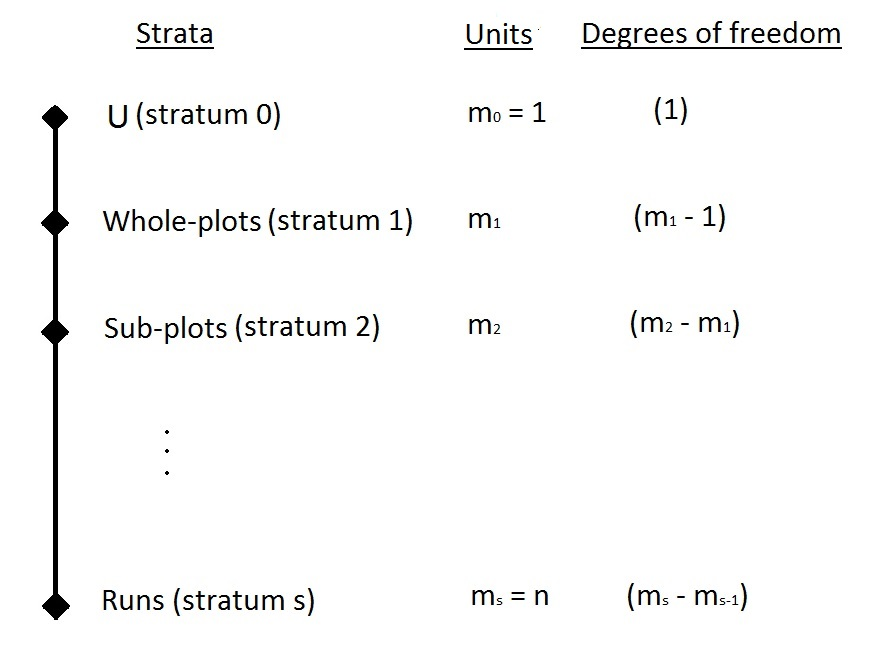
\includegraphics[scale=0.85]{Hasse.jpg}      %width=\textwidth
\caption{Hasse diagram for factors}
\label{Fig::Hasse}
\end{center}
\end{figure} 
 
Recall the expression for the linear polynomial hierarchical model from (\ref{eq::intro_ms}):
\begin{equation}
\label{eq::back_ms}
\bm{Y}=\bm{X}\bm{\beta}+\sum_{i=1}^{s}\bm{Z}_{i}\bm{\varepsilon}_{i},
\end{equation} 
where the first part $\bm{X\beta}$ contains the fixed effects, and $\sum_{i=1}^{s}\bm{Z}_{i}\bm{\varepsilon}_{i}$ stands for the random part, i.e.~it comprises information on variation occurring at each level of randomisation. All of the errors are assumed to be independent, having zero means and constant variances $\sigma^2_{i}$ and, as seen from the model formulation, additive.

In this case the fixed effects coefficients, $\bm{\beta}$ are usually estimated using the Generalised Least Square (GLS) formula:
\begin{equation}
\label{eq::back_gls}
\bm{\hat{\beta}}=(\bm{X}'\bm{VX})^{-1}\bm{X}'\bm{V}^{-1}Y,
\end{equation}
so that the variance of the estimators is
\begin{equation}
\label{eq::back_glsvar}
Var(\bm{\hat{\beta}})=(\bm{X}'\bm{VX})^{-1},
\end{equation}
where $\bm{V}$ is the variance-covariance matrix of the (normally distributed) responses, has a block-diagonal structure, and can be presented as:
\begin{equation}
\label{eq::back_glsV}
\bm{V}=\sum_{i=1}^{s}\sigma^2_{i}\bm{Z}_{i}\bm{Z}'_{i}=\sigma^{2}_{s}\left(\bm{I}_{n}+\sum_{i=1}^{s-1}\eta_{i}\bm{Z}_{i}\bm{Z}'_{i}\right).
\end{equation}
Here $\eta_{i}=\sigma^{2}_{i}/\sigma^{2}_{s}$ is defined as a variance ratio, denoting the magnitude of variability occurring at higher strata scaled with respect to the between-run variance.

At the analysis stage, as the variance components are unknown, their estimates are obtained and substituted in (\ref{eq::back_glsvar}) to obtain an estimated variance-covariance matrix of the parameters' estimators, $\bm{\hat{V}(\hat{\beta})}$; the estimation methods are discussed in more detail in Chapter \ref{ch::mse_ms}.

However, when an experiment is being planned, and none of the $\eta_{i}$ or $\sigma^2_{s}$ are known, there are two main approaches to deal with it. The first one is to search for designs assuming some point prior values of the $\eta$ parameter and, for these, evaluate the variance-based criteria, considering all strata simultaneously.

The case of split-plot experiments, with two strata, $\sigma^2_{s}=\sigma^2$ and $\eta=\sigma^2_{1}/\sigma^2$, has been extensively considered in the literature. \cite{Goos2001Doptimal} considered the three cases when D-optimal designs for split-plot experiments do not depend on the value of $\eta$; in other practical cases an estimate of the variance ratio is to be provided. \cite{Goos2003Doptimal} and \cite{Jones2007candidate} developed algorithms for finding $D$-optimal split-plot designs and for some examples demonstrated the robustness to the different values of $\eta$. An algorithm for constructing $D$-optimal split-split-plot designs can be found in the paper by \cite{Jones2009Doptimal}. 
%\cite{Goos2007tailor} -- split-plot for mixture experiments  

The Bayesian alternative to the `exhaustive search' approach across the unknown parameter space allows specifying a prior distribution on the unknown parameters, and then evaluating the criteria by integrating over that prior. \cite{Arnouts2012staggered} presented a coordinate-exchange algorithm for constructing D-optimal designs for a staggered experimental structure (i.e. values of hard-to-change factors' are changed at different time points), with log-normal prior distributions being put on the variance ratios. Later \cite{Arnouts2015staggered} studied the staggered structured designs in the context of response surface modelling, and considered a few examples of D- and I-optimal designs.
 
\cite{Mylona2014optimal} introduced a composite criterion, combining $D$-optimality for the fixed and variance components; in such an approach both the criterion formula and the form of the prior distributions define the way of evaluation the criterion function, which often leads to the necessity of choosing a computationally efficient numerical methodology. \cite{Gilmour2009analysis} proposed an appropriate Bayesian analysis strategy of data from multistratum experiments, that is robust to designs non-orthogonality and is shown to be more reliable than REML approach.  

However, in the general case a lot of computational effort might be required in order to be confident in the goodness of the design obtained by choosing from a set of assumed possible values of $\eta_i$, either using point priors or adapting general Bayesian strategy, especially when there are more than two strata and, therefore, the range of unknown parameters becomes multi-dimensional. The stratum-by-stratum approach (as first suggested by \cite{Trinca2001multistratum} and more recently improved by \cite{Trinca2015improved}) implies going from the highest stratum to the lowest, at each level choosing the set of treatments, and the units of higher level being treated as fixed block effects. Such methodology allows `protecting' against the case of large higher level variances, and eliminates the need for any prior information on unknown parameters. The authors later adapted the stratum-by-stratum  strategy for the inference criteria \citep{Trinca2016SPinference}, providing tools for constructing efficient designs for relatively small experiments in the presence of restricted randomisation.

\section{Accounting for Model Misspecification}
\label{sec::back_misspecification}
Standard optimality criteria usually rely on the assumption that the fitted model provides a (significantly) good fit for the data. However, as in many experiments this might be a concern, the possibility of model misspecification should be accounted for at the stage of planning. 

Lots of research has been conducted in this direction. In the cases when the form of model contamination is unknown, some authors adapt the approach of incorporating some prior knowledge regarding the possible functions representing the model departure from the data, for example, \cite{Notz1989Optimal} presented the methodology of optimal planning (with respect to the fitted model coefficients' estimates) while accounting for a presence of a bias function (that has $0$ expectation over the prior and finite second moment). In a similar view \cite{Wiens1993Designs} studied the construction of designs that minimise the effect of the unknown disturbance on the coverage probability of the confidence ellipsoid of the fitted model's parameters. \cite{Allen2003Experimental} proposed the expected integrated mean-squared error optimality criterion for maximising the prediction precision in the presence of potential model misspecification; \cite{Woods2005designing} accounted for (involving) a random additive model contamination in their optimality criteria for polynomial spline regression models.

When the form of the model deviation is assumed to be known, one of the most particular cases is when the fitted model is nested within the full one, and both of them are estimable; essentially the initial problem is reduced to model discrimination. One of the basic approaches for choosing between two polynomial models is $T$ -- optimality, the criterion first introduced by \cite{Atkinson1975Design} for discriminating between any two polynomials; a lot of research has been conducted based on this, e.g. \cite{Dette2012T} focused on constructing $T$-optimal designs when polynomials differ in degree by two. \cite{Dette1995Optimal} introduced a more general strategy of constructing designs optimal with respect to identifying the best suitable degree of the polynomial model to be fitted.

A series of works has been devoted to constructing designs such that their desirable properties would be robust to possible faults in model choice. For example, \cite{Wiens1992Minimax} introduced the minimax approach to the class of loss function that the author defined as monotonic functions of the mean squared error matrix ocurring from the model misspecification function coming from a bounded in $\mathcal{L}_2$ set. Later \cite{Wiens2009Robust} developed a general methodology of finding optimal sequential designs allowing for model discrimination and then, after the best model has been chosen, for efficient parameter estimation and/or prediction. \cite{Wiens2000Bias} aimed at minimising the maximum integrated mean squared error of the fitted values, where the maximum is found over the functional family of model deviations. 

The $\mathcal{Q}_{B}$ criterion, first introduced by \cite{Tsai2007Three}, aimed at taking advantage of experimenter's prior knowledge and providing efficient estimations of all models nested within the ``maximal model of interest'', was later generalised by \cite{Tsai2010General} and shown to be interpretable and statistically meaningful. \cite{Smucker2012Model} were the first ones to consider split-plot structures in this context; they introduced a `weighted' adaptation of $D$-optimality in order to obtain designs accounting not for one, but for a set of models.

In this thesis, due to the primary interest being the quality of inference, the view of model uncertainty will be strongly based on the approach developed by \cite{Goos2005model}, combining model-robust and model-sensitive approaches to design construction; it is examined in more detail in Chapter \ref{ch::generalised}. 

\section{Search Implementation: Point-Exchange Algorithm}

As mentioned above, in practice we work with exact designs, and there are quite a few options of how this search should be implemented.  

The design search methodology for a factorial experiment used here was first introduced in \citet{fedorov1972theory}. The candidate set of points is composed as the set of all possible combinations of the factors' levels. The algorithm starts with generating a random design from this set and, starting with the very first point in it, it goes through the candidate set, exchanges the current point in the current design with the `new' point from the candidate set and if the exchange improves the value of the criterion function, keeps the exchange. A number of random starts is usually set up, and the best design is kept in the end.

The coordinate-exchange algorithm, as a possible alternative, was first introduced by \cite{Meyer1995Coordinate} and since then has been widely used by various authors when searching for exact designs. It starts with generating a random initial design, and, as going through rows and columns of design matrix, the values of each element of the design matrix are being swapped among all the candidate values for the corresponding factor, and the criterion is evaluated; this is done till no improvement is achieved, and again, the whole procedure is repeated for some number of random starts. 

The obvious advantage is that there is no candidate set of design points required. It is more popular in experiments with hierarchical unit structures: \cite{Jones2007candidate} adapted the approach for constructing split-plot D-optimal designs, whilst \cite{Sambo2014Coordinate} proposed the coordinate-exchange two-phase local search (CE-TPLS), allowing simultaneous optimisation with respect to $D$- and $I$-optimality. Later \cite{Borrotti2016Multi} introduced the coordinate-exchange algorithm, now for multistratum design search and for several objectives (up to six optimality criteria), such that the whole Pareto front can be considered and the best design chosen.  

When working with multistratum designs, we essentially adopt the stratum-by-stratum approach presented by \cite{Trinca2016SPinference}, as further described in Chapter \ref{ch::mse_ms}. 

%%%%%%  




